\documentclass[../main.tex]{subfiles}
\graphicspath{{\subfix{../images/}}} % Images path

\begin{document}

\section{Results}\label{sec:results}

The results obtained with all the classifiers, the two feature extraction
methods and the different image representations are summarized in
Table~\ref{tab:results} while Figure~\ref{fig:classifiers-comparison} compares
the results for the grid sampling method.\\
The average accuracy over all the classes has been used as the main assessment
metric for all the models. 
All the experimental results have been obtained by running the models on a machine equipped with an Intel\textsuperscript{\textregistered}~Core\textsuperscript{TM}~i7--8565U CPU @ $\SI{4.60}{\giga\hertz}$ and $\SI{8}{\giga\byte}$ of RAM.\\
The dummy classifier, that always predicts the most frequent class  (\itt{OpenCountry}) on the test set, has been used as baseline for comparison
for the other models and the average accuracy it achieved is $\SI{10.39}{\percent}$.\\
% Before analyzing the performance of the single classifiers, 
First of all, it's possible to notice that the results obtained using grid sampling consistently surpass the ones resulting from the SIFT detector. This confirms the idea presented in \itt{Fei-Fei and Perona}~\cite{feifei} and \itt{Lazebnik et al.}~\cite{lazebnik} for which grid sampling works better for scene classification tasks, as it allows to capture uniform regions such as sky, water, or road surfaces that might be crucial in discriminating between classes.\\
Looking at the performance of the different classifiers instead, the KNN ones
surpassed the baseline, recording average accuracies
between $\SI{40}{\percent}$ and $\SI{50}{\percent}$ with a small gain in
performance given by the multiple neighbors approach over the single
neighbor classifier.\\
Undoubtably, much better results have been achieved by the SVM
classifiers with accuracies ranging from $\SI{50}{\percent}$ to
$\SI{70}{\percent}$.
In particular, the adoption of specialized kernels significantly boosted the
performance of the SVM classifiers, at least in the \itt{HIST} and \itt{TF-IDF}
representations.
Indeed, the $\SI{71.42}{\percent}$ accuracy obtained with the $\chi^2$ kernel
and the $\SI{70.62}{\percent}$ with the intersection one are in agreement with
the findings of \itt{Van Gemert et al.}~\cite{gemert} for the hard assignment
case.\\
However, from the comparison of the different image representation techniques it
emerges that, while little to no differences are observed between the
\itt{HIST} and \itt{TF-IDF} representations, the implementation of the soft
assignment techniques failed in improving the classification performances as
reported in \itt{Van Gemert et al.}~\cite{gemert}, except for some
isolated cases. In contrast with the results of the paper, the accuracies
measured for these representations are mostly comparable, if not worse with respect
to the ones of the hard assignment cases.\\
A further level of assessment is also given by the confusion matrices computed
for all the classifiers\footnote{Only for \itt{HIST} representation and grid
	sampling method as explained in appendix~\ref{app:confusion-matrices}.} and reported in appendix~\ref{app:confusion-matrices}.
These, not only confirm the superiority of the SVM classifiers with respect to
the KNN ones, but also highlight the most difficult scenes to
recognize. In detail, in most of the classifiers a noticeable
(but understandable) confusion arises between the \itt{Open Country} and
\itt{Coast} classes as well as among the \itt{LivingRoom}, \itt{Bedroom},
\itt{Kitchen} and \itt{Office} classes. Consistently, the hardest scene
to classify has been the \itt{Industrial} one, which matches with the results
from literature.\\
By far, the best accuracy has been obtained by the SVM classifiers
using the spatial pyramid matching approach. In this case, the combination of  sampling features
from a regular grid and adopting the \itt{SPM} representation for the images
allowed to achieve an accuracy of $\SI{75.54}{\percent}$. This result is
significantly better than the other classifiers and is a clear indication that
the spatial information is crucial for the scene recognition task. The
superiority of this approach is also confirmed by the almost completely diagonal
confusion matrix (Figure~\ref{fig:confusion-matrix-pmk}), in which only few of
the previous misclassifications remain, mainly between the \itt{Living Room} and
\itt{Bedroom} classes. Although higher than the other classifiers, the lowest
accuracy is still measured for the \itt{Industrial} class.\\

\begin{table}[htb]
  \renewcommand{\arraystretch}{1.3} % Row height
  \centering
  \begin{tabular}{|c|c|c|c|}

    % Header (different color)
    \hline
    % \rowcolor{boxcolor}
    \multirow{2}{*}{\textbf{Classifier}} &
    \multirow{2}{*}{\textbf{Image Representation}} &
    \multicolumn{2}{c|}{\textbf{Feature Extraction}} \\
    \cline{3-4}
    & & \itt{SIFT detector} & \itt{Grid sampling} \\

    % Rows
	\cline{1-4}
    \hline
		\multirow{5}{*}{Dummy Classifier} & 
		\itt{HIST} & \SI{10.39}{\percent} & \SI{10.39}{\percent} \\
		\cline{2-4}
		& \itt{TF-IDF} & \SI{10.39}{\percent} & \SI{10.39}{\percent} \\
		\cline{2-4}
		& \itt{KCB} & \SI{10.39}{\percent} & \SI{10.39}{\percent} \\
		\cline{2-4}
		& \itt{UNC} & \SI{10.39}{\percent} & \SI{10.39}{\percent} \\
		\cline{2-4}
		& \itt{PLA} & \SI{10.39}{\percent} & \SI{10.39}{\percent} \\
	\cline{1-4}
	\hline
		\multirow{5}{*}{1-NN} &
		\itt{HIST} & \SI{31.49}{\percent} & \SI{43.75}{\percent} \\
		\cline{2-4}
		& \itt{TF-IDF} & \SI{31.83}{\percent} & \SI{39.30}{\percent} \\
		\cline{2-4}
		& \itt{KCB} & \SI{33.40}{\percent} & \SI{45.53}{\percent} \\
		\cline{2-4}
		& \itt{UNC} & \SI{35.38}{\percent} & \SI{49.01}{\percent} \\
		\cline{2-4}
		& \itt{PLA} & \SI{36.72}{\percent} & \SI{47.07}{\percent} \\
	\cline{1-4}
	\hline
		\multirow{5}{*}{k-NN} &
		\itt{HIST} & \SI{37.19}{\percent} & \SI{43.95}{\percent} \\
		\cline{2-4}
		& \itt{TF-IDF} & \SI{36.42}{\percent} & \SI{42.18}{\percent} \\
		\cline{2-4}
		& \itt{KCB} & \SI{38.93}{\percent} & \SI{50.69}{\percent} \\
		\cline{2-4}
		& \itt{UNC} & \SI{42.31}{\percent} & \SI{53.94}{\percent} \\
		\cline{2-4}
		& \itt{PLA} & \SI{43.05}{\percent} & \SI{54.77}{\percent} \\
	\cline{1-4}
	\hline
		\multirow{5}{*}{SVM (RBF)} &
		\itt{HIST} & \SI{50.65}{\percent} & \SI{66.43}{\percent} \\
		\cline{2-4}
		& \itt{TF-IDF} & \SI{50.89}{\percent} & \SI{62.65}{\percent} \\
		\cline{2-4}
		& \itt{KCB} & \SI{54.77}{\percent} & \SI{60.87}{\percent} \\
		\cline{2-4}
		& \itt{UNC} & \SI{56.08}{\percent} & \SI{64.86}{\percent} \\
		\cline{2-4}
		& \itt{PLA} & \SI{51.39}{\percent} & \SI{65.13}{\percent} \\
	\cline{1-4}
	\hline
		\multirow{5}{*}{SVM ($\chi^2$)} &
		\itt{HIST} & \SI{52.66}{\percent} & \SI{71.42}{\percent} \\
		\cline{2-4}
		& \itt{TF-IDF} & \SI{52.03}{\percent} & \SI{70.22}{\percent} \\
		\cline{2-4}
		& \itt{KCB} & \SI{53.94}{\percent} & \SI{60.03}{\percent} \\
		\cline{2-4}
		& \itt{UNC} & \SI{54.37}{\percent} & \SI{63.05}{\percent} \\
		\cline{2-4}
		& \itt{PLA} & \SI{45.06}{\percent} & \SI{58.46}{\percent} \\
	\cline{1-4}
	\hline
		\multirow{5}{*}{SVM ($\cap$)} &
		\itt{HIST} & \SI{50.95}{\percent} & \SI{70.62}{\percent} \\
		\cline{2-4}
		& \itt{TF-IDF} & \SI{50.79}{\percent} & \SI{68.91}{\percent} \\
		\cline{2-4}
		& \itt{KCB} & \SI{52.23}{\percent} & \SI{60.34}{\percent} \\
		\cline{2-4}
		& \itt{UNC} & \SI{53.37}{\percent} & \SI{63.79}{\percent} \\
		\cline{2-4}
		& \itt{PLA} & \SI{49.15}{\percent} & \SI{60.47}{\percent} \\
	\cline{1-4}
	\hline
		\makecell{SVM\\ (\itt{Spatial Pyramid})} & \itt{SPM} & --- & \SI{75.54}{\percent} \\
	\cline{1-4}
	\hline

  \end{tabular}
  \caption{Average accuracies for all the implemented classifiers comparing feature extraction methods and image representations.}\label{tab:results}
  \renewcommand{\arraystretch}{1} % Reset row height to default
\end{table}

\begin{figure}[htb]
  \centering
  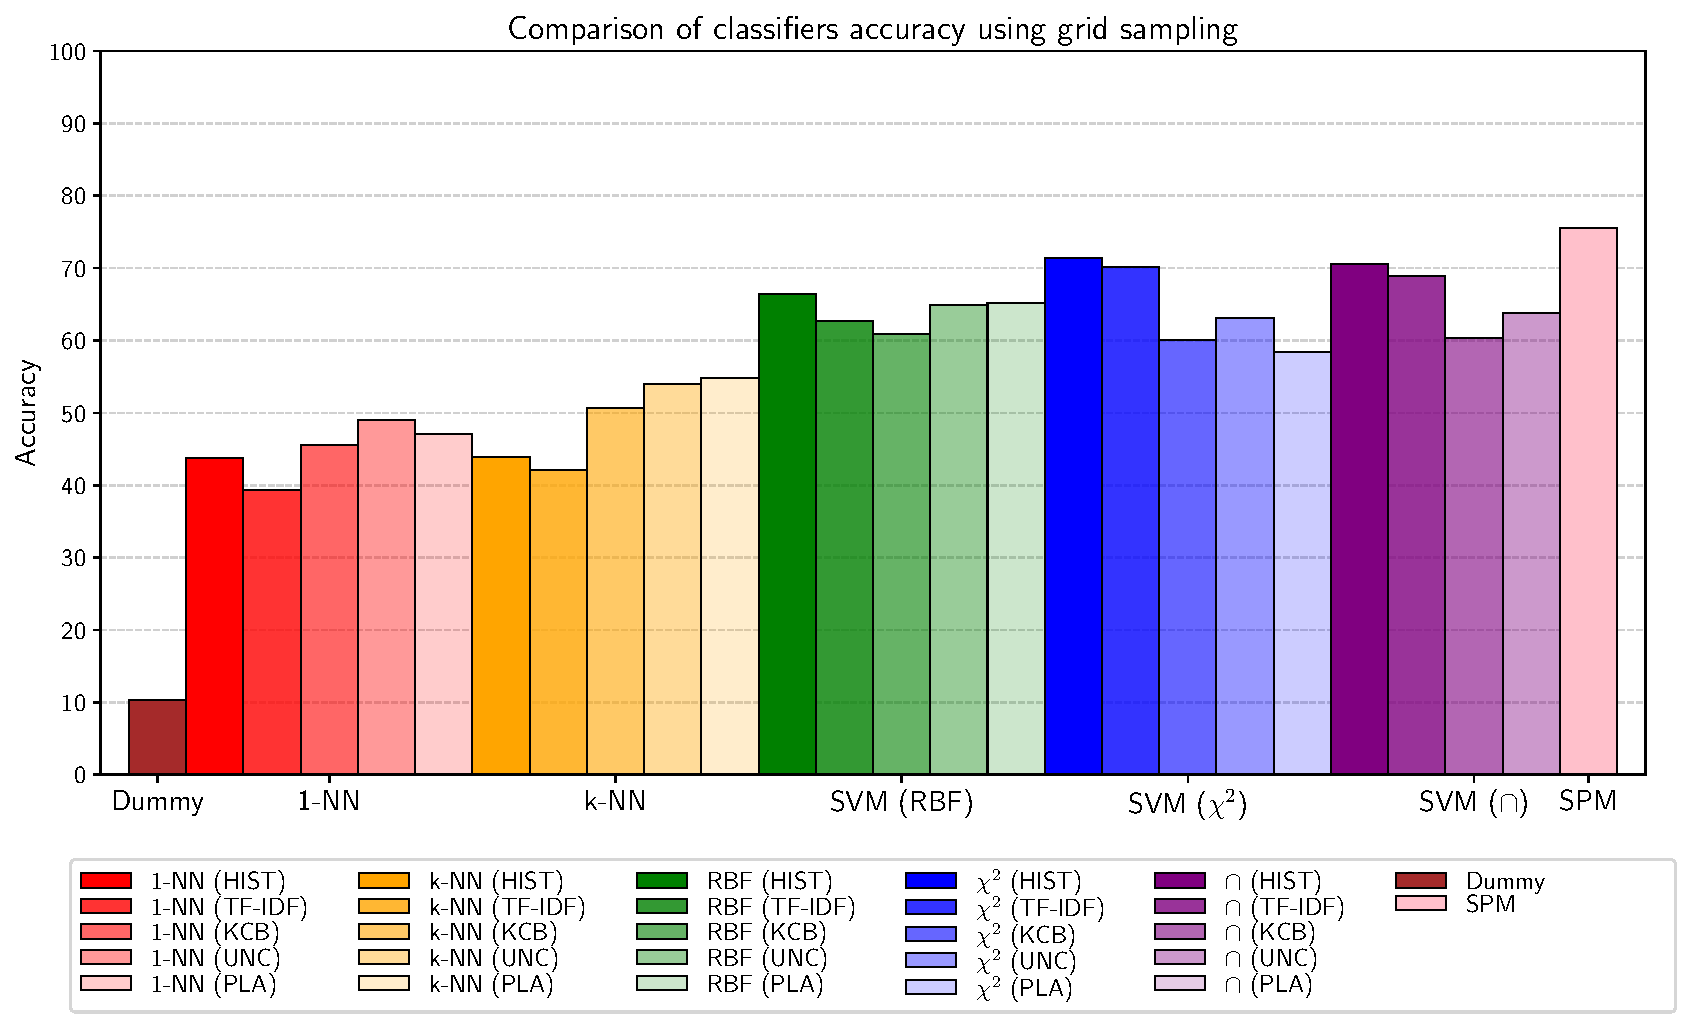
\includegraphics[width=\textwidth]{classifiers_accuracy.pdf}
  \caption{Comparison of the classifiers accuracies using grid sampling.}\label{fig:classifiers-comparison}
\end{figure}

\end{document}
